\documentclass[11pt, oneside]{book}

%%%%%%%%%%%%%%Include Packages%%%%%%%%%%%%%%%%%%%%%%%%%%
\usepackage{xcolor}
\usepackage{mathtools}
\usepackage[a4paper, total={6in, 8in}, margin=1.25in]{geometry}
\usepackage{amsmath}
\usepackage{amssymb}
\usepackage{paralist}
\usepackage{rsfso}
\usepackage{amsthm}
\usepackage{wasysym}
\usepackage[inline]{enumitem}   
\usepackage{hyperref}
\usepackage{tocloft}
\usepackage{wrapfig}
\usepackage{titlesec}
\usepackage{colortbl}
\usepackage{stackengine} 
\usepackage{listings}
%%%%%%%%%%%%%%%%%%%%%%%%%%%%%%%%%%%%%%%%%%%%%%%%%%%%%%%%



%%%%%%%%%%%%%%%Code%%%%%%%%%%%%%%%%%%%%%%%%%%%%%%%%%%%%%
\definecolor{codegreen}{rgb}{0,0.6,0}
\definecolor{codegray}{rgb}{0.5,0.5,0.5}
\definecolor{codepurple}{rgb}{0.58,0,0.82}
\definecolor{backcolour}{rgb}{0.95,0.95,0.92}

\lstdefinestyle{mystyle}{
    backgroundcolor=\color{backcolour},   
    commentstyle=\color{codegreen},
    keywordstyle=\color{magenta},
    numberstyle=\tiny\color{codegray},
    stringstyle=\color{codepurple},
    basicstyle=\ttfamily\footnotesize,
    breakatwhitespace=false,         
    breaklines=true,                 
    captionpos=b,                    
    keepspaces=true,                 
    numbers=left,                    
    numbersep=5pt,                  
    showspaces=false,                
    showstringspaces=false,
    showtabs=false,                  
    tabsize=2
}
%%%%%%%%%%%%%%%%%%%%%%%%%%%%%%%%%%%%%%%%%%%%%%%%%%%%%%%%

%%%%%%%%%%%%%%%Chapter Setting%%%%%%%%%%%%%%%%%%%%%%%%%%
\definecolor{gray75}{gray}{0.75}
\newcommand{\hsp}{\hspace{20pt}}
\titleformat{\chapter}[hang]{\Huge\bfseries}{\thechapter\hsp\textcolor{gray75}{$\mid$}\hsp}{0pt}{\Huge\bfseries}
%%%%%%%%%%%%%%%%%%%%%%%%%%%%%%%%%%%%%%%%%%%%%%%%%%%%%%%%

%%%%%%%%%%%%%%%%%Theorem environments%%%%%%%%%%%%%%%%%%%
\newtheoremstyle{break}
  {\topsep}{\topsep}%
  {\itshape}{}%
  {\bfseries}{}%
  {\newline}{}%
\theoremstyle{break}
\theoremstyle{break}
\newtheorem{axiom}{Axiom}
\newtheorem{thm}{Theorem}[section]
\renewcommand{\thethm}{\arabic{section}.\arabic{thm}}
\newtheorem{lem}{Lemma}[thm]
\newtheorem{cor}{Corollary}[thm]
\newtheorem{defn}{Definition}[thm]
\newenvironment{indEnv}[1][Proof]
  {\proof[#1]\leftskip=1cm\rightskip=1cm}
  {\endproof}
%%%%%%%%%%%%%%%%%%%%%%%%%%%%%%%%%%%%%%%%%%%%%%%%%%%%%%


%%%%%%%%%%%%%%%%%%%%%%%Integral%%%%%%%%%%%%%%%%%%%%%%%
\def\upint{\mathchoice%
    {\mkern13mu\overline{\vphantom{\intop}\mkern7mu}\mkern-20mu}%
    {\mkern7mu\overline{\vphantom{\intop}\mkern7mu}\mkern-14mu}%
    {\mkern7mu\overline{\vphantom{\intop}\mkern7mu}\mkern-14mu}%
    {\mkern7mu\overline{\vphantom{\intop}\mkern7mu}\mkern-14mu}%
  \int}
\def\lowint{\mkern3mu\underline{\vphantom{\intop}\mkern7mu}\mkern-10mu\int}
%%%%%%%%%%%%%%%%%%%%%%%%%%%%%%%%%%%%%%%%%%%%%%%%%%%%%%



\newcommand{\R}{\mathbb{R}}
\newcommand{\N}{\mathbb{N}}
\newcommand{\Z}{\mathbb{Z}}
\newcommand{\Q}{\mathbb{Q}}
\newcommand{\C}{\mathbb{C}}
\newcommand{\T}{\mathcal{T}}
\newcommand{\M}{\mathcal{M}}
\newcommand{\Symm}{\text{Symm}}
\newcommand{\Alt}{\text{Alt}}
\newcommand{\Int}{\text{Int}}
\newcommand{\Bd}{\text{Bd}}
\newcommand{\Power}{\mathcal{P}}
\newcommand{\ee}[1]{\cdot 10^{#1}}
\newcommand{\spa}{\text{span}}
\newcommand{\sgn}{\text{sgn}}
\newcommand{\degr}{\text{deg}}
\newcommand{\pd}{\partial}
\newcommand{\that}[1]{\widetilde{#1}}
\newcommand{\lr}[1]{\left(#1\right)}
\newcommand{\vmat}[1]{\begin{vmatrix} #1 \end{vmatrix}}
\newcommand{\bmat}[1]{\begin{bmatrix} #1 \end{bmatrix}}
\newcommand{\pmat}[1]{\begin{pmatrix} #1 \end{pmatrix}}
\newcommand{\rref}{\xrightarrow{\text{row\ reduce}}}
\newcommand{\txtarrow}[1]{\xrightarrow{\text{#1}}}
\newcommand\oast{\stackMath\mathbin{\stackinset{c}{0ex}{c}{0ex}{\ast}{\Circle}}}
\newcommand{\txt}{Wald's \textit{General Relativity}}

\newcommand{\note}{\color{red}Note: \color{black}}
\newcommand{\remark}{\color{blue}Remark: \color{black}}
\newcommand{\example}{\color{green}Example: \color{black}}
\newcommand{\exercise}{\color{green}Exercise: \color{black}}

%%%%%%%%%%%%%%%%%%%%%%Roman Number%%%%%%%%%%%%%%%%%%%%%%%
\makeatletter
\newcommand*{\rom}[1]{\expandafter\@slowromancap\romannumeral #1@}
\makeatother
%%%%%%%%%%%%%%%%%%%%%%%%%%%%%%%%%%%%%%%%%%%%%%%%%%%%%%%%%

%%%%%%%%%%%%%table of contents%%%%%%%%%%%%%%%%%%%%%%%%%%%%
%\setlength{\cftchapindent}{0em}
%\cftsetindents{section}{2em}{3em}
%
%\renewcommand\cfttoctitlefont{\hfill\huge\bfseries}
%\renewcommand\cftaftertoctitle{\hfill\mbox{}}
%
%\setcounter{tocdepth}{2}
%%%%%%%%%%%%%%%%%%%%%%%%%%%%%%%%%%%%%%%%%%%%%%%%%%%%%%%%%%


%%%%%%%%%%%%%%%%%%%%%Footnotes%%%%%%%%%%%%%%%%%%%%%%%%%%%
\newcommand\blfootnote[1]{%
  \begingroup
  \renewcommand\thefootnote{}\footnote{#1}%
  \addtocounter{footnote}{-1}%
  \endgroup
}
%%%%%%%%%%%%%%%%%%%%%%%%%%%%%%%%%%%%%%%%%%%%%%%%%%%%%%%%%

%%%%%%%%%%%%%%%%%%%%%Section%%%%%%%%%%%%%%%%%%%%%%%%%%%%%
\makeatletter
\def\@seccntformat#1{%
  \expandafter\ifx\csname c@#1\endcsname\c@section\else
  \csname the#1\endcsname\quad
  \fi}
\makeatother
%%%%%%%%%%%%%%%%%%%%%%%%%%%%%%%%%%%%%%%%%%%%%%%%%%%%%%%%%

%%%%%%%%%%%%%%%%%%%%%%%%%%%%%%%%%%%Enumerate%%%%%%%%%%%%%%
\makeatletter
% This command ignores the optional argument 
% for itemize and enumerate lists
\newcommand{\inlineitem}[1][]{%
\ifnum\enit@type=\tw@
    {\descriptionlabel{#1}}
  \hspace{\labelsep}%
\else
  \ifnum\enit@type=\z@
       \refstepcounter{\@listctr}\fi
    \quad\@itemlabel\hspace{\labelsep}%
\fi}
\makeatother
\parindent=0pt
%%%%%%%%%%%%%%%%%%%%%%%%%%%%%%%%%%%%%%%%%%%%%%%%%%%%%%%%%%



\begin{document}

	\begin{titlepage}
		\begin{center}
			\vspace*{0.5cm}
			\Huge \color{red}
				\textbf{Homework 4}\\
			\vspace{0.5cm}			
			\Large \color{black}
			Physics 542 - Quantum Optics\\
			Professor Alex Kuzmich
			\vspace{1.5cm}

			
\includegraphics[scale=1.15]{hmm.pdf}
			
			
			\vspace{2cm}
			\LARGE
				\textbf{Jinyan Miao}\\
				\hfill\break
				\LARGE Fall 2023\\
			\vspace{1cm}

		\vspace*{\fill}
		\end{center}			
	\end{titlepage}

\chapter{}
Here we suppose that the right eigenstate of the creation operator exists, that is, we write
\begin{align*}
\hat{a}^\dagger |m\rangle = m |m\rangle\,,
\end{align*}
for some $m \in \C$. We can write $|m\rangle$ as superposition of the usual basis,
\begin{align*}
|m\rangle = \sum_{n=0}^\infty c_n |n\rangle\,.
\end{align*}
Then we must have
\begin{align*}
\hat{a}^\dagger |m\rangle =\sum_{n=0}^\infty c_n \,\hat{a}^\dagger |n\rangle = \sum_{n=0}^\infty c_n \sqrt{n+1}\, | n+1\rangle\,.
\end{align*}
On the other hand, 
\begin{align*}
\hat{a}^\dagger |m\rangle =m|m\rangle = \sum_{n=0}^\infty c_n m |n\rangle = \sum_{n=0}^\infty c_n \sqrt{n+1}\, | n+1\rangle\,.
\end{align*}
As $\langle n_1 |n_2\rangle =0$ for $n_1\neq n_2$, thus we conclude that we have $c_0 = 0$, and 
\begin{align*}
c_{n+1} = \frac{c_n \sqrt{n+1}}{m}\,.
\end{align*}
As $c_0 = 0$, we thus require $c_n = 0$ for all $n \in \N$, so we have $|m\rangle = 0$, such a state does not exist. 

\chapter{}
For coherent state $|\beta\rangle$, we first compute
\begin{align}
C_N(\lambda) = \text{tr}(\hat{\rho} e^{\lambda \hat{a}^\dagger}e^{-\lambda^* \hat{a}}) = \langle \beta | e^{\lambda \hat{a}^\dagger}e^{-\lambda^* \hat{a}} | \beta\rangle = e^{\lambda^* \hat{a}}\langle \beta | e^{-\lambda^* \hat{a}}|\beta \rangle =\langle e^{\lambda^* \beta} \beta | e^{-\lambda^* \beta}\beta \rangle = e^{\lambda \beta^* - \lambda ^*\beta}\,.  
\end{align}
Now we compute
\begin{align*}
W(\alpha) 
&= \frac{1}{\pi^2}\int e^{\lambda^* \alpha - \lambda \alpha^*} \, C_N(\lambda) \, e^{-|\lambda|^2/2}\, d^2 \lambda\\
&= \frac{1}{\pi^2}\int e^{\lambda^* \alpha - \lambda \alpha^*} \, e^{\lambda \beta^* - \lambda ^*\beta} \, e^{-|\lambda|^2/2}\, d^2 \lambda\\
&= \frac{1}{\pi^2}\int e^{\lambda^* \alpha - \lambda \alpha^*+\lambda \beta^* - \lambda ^*\beta-|\lambda|^2/2}\, d^2 \lambda\\
&= \frac{1}{\pi^2}\int e^{\lambda^*(\alpha-\beta) - \lambda(\alpha^*-\beta^*)
-|\lambda|^2/2}\, d^2 \lambda\\
&= \frac{1}{\pi^2}\int_0^\infty \int_0^{2\pi}  \exp(rs e^{-i (\theta-\phi)} - r s e^{i(\theta-\phi)} - r^2/2)\, r\, d\theta\, dr\\
&= \frac{1}{\pi^2}\int_0^\infty \int_0^{2\pi} e^{-2i rs \sin(\theta- \phi)}\, d\theta\,  e^{-r^2/2}\, r \, dr\\
&= \frac{2}{\pi}\int_0^\infty J_0(2rs) \, e^{-r^2/2}\, r\, dr\\
&=  \frac{2}{\pi}\, e^{-2s^2}\\
&= \frac{2}{\pi}e^{-2|\alpha-\beta|^2}\,,
\end{align*}
where we have abbreviated $\lambda = re^{i\theta}$ and $\alpha-\beta = se^{i\phi}$ and the last integral is computed via Eq.\ (4) in Erdelyi's \textit{Tables of Integral Transforms} vol II, p.\ 13. 

\newpage
Now we consider the number state $|n\rangle$. We first compute
\begin{align*}
C_N(\lambda) = \langle n | e^{\lambda \hat{a}^\dagger}e^{-\lambda^* \hat{a}}|n\rangle &= \sum_{i=0}^\infty \sum_{j=0}^\infty \langle n | \frac{\lambda^i (\hat{a}^{\dagger})^i}{i!}\frac{(-1)^j (\lambda^*)^j \hat{a}^j}{j!} |n\rangle\\
&= \sum_{i=0}^\infty \sum_{j=0}^\infty\frac{(-1)^j\lambda^{i}(\lambda^*)^j }{i!\,j!}  \langle n | (\hat{a}^{\dagger})^i\hat{a}^j |n\rangle\\
&= \sum_{i=0}^\infty \sum_{j=0}^\infty\frac{(-1)^j\lambda^{i}(\lambda^*)^j }{i!\,j!}  \hat{a}^i\langle n | \hat{a}^j |n\rangle\\
&= \sum_{i=0}^n \frac{(-1)^i |\lambda|^{2i}}{i!\,i!}\frac{n!}{(n-i)!}\\
&= L_n(|\lambda|^2)\,.
\end{align*}
Then we compute
\begin{align*}
W(\alpha) 
&= \frac{1}{\pi^2}\int e^{\lambda^* \alpha - \lambda \alpha^*}L_n(|\lambda|^2) \, e^{-|\lambda|^2/2}\, d^2\lambda\\
&= \frac{1}{\pi^2}\int e^{\lambda^* \alpha - \lambda \alpha^* - |\lambda|^2/2}L_n(|\lambda|^2) \, d^2\lambda\\
&= \frac{1}{\pi^2}\int_0^\infty \int_0^{2\pi} L_n(r^2) \, \exp(rs e^{-i (\theta-\phi)} - r s e^{i(\theta-\phi)} - r^2/2)\, r\, d\theta\, dr\\
&= \frac{1}{\pi^2}\int_0^\infty \int_0^{2\pi} e^{-2i rs \sin(\theta- \phi)}\, d\theta\, L_n(r^2) e^{-r^2/2}\, r \, dr\\
&= \frac{2}{\pi}\int_0^\infty J_0(2rs)\, L_n(r^2) \, e^{-r^2/2}\, r\, dr\\
&= (-1)^n \frac{2}{\pi}\, e^{-2s^2}\, L_n(4s^2)\\
&= (-1)^n \frac{2}{\pi}\, e^{-2|\alpha|^2}\, L_n(4|\alpha|^2)\,,
\end{align*}
where we have abbreviated $\lambda = re^{i\theta}$ and $\alpha = se^{i\phi}$ and the last integral is computed via Eq.\ (4) in Erdelyi's \textit{Tables of Integral Transforms} vol II, p.\ 13. 

\chapter{}
Here we consider the superposition of coherent states $|\pm \beta\rangle$, 
\begin{align*}
|\Psi\rangle = \frac{1}{\sqrt{
2}}\left( |\beta\rangle + |-\beta\rangle\right)\,.
\end{align*}
\textbf{(a)} Here we see that we have
\begin{align*}
\langle \Psi |\Psi\rangle = \frac{1}{2}\left( \langle \beta |\beta\rangle + \langle -\beta |-\beta\rangle + \langle -\beta |\beta\rangle + \langle \beta |-\beta\rangle\right) = \frac{1}{2}\left( 2 + 2e^{-2|\beta|^2}\right)\,.
\end{align*}
For large enough $|\beta|^2 \gg 1$, $e^{-2|\beta|^2} \sim 0$, it follows that $\langle \Psi|\Psi\rangle = 1$. \\

\textbf{(b)} Here we simply compute
\begin{align*}
\langle n |\Psi\rangle = \frac{1}{\sqrt{2}}\left( \langle n |\beta\rangle - \langle n |-\beta\rangle\right) = \frac{e^{-|\beta|^2/2}}{\sqrt{2}}\left(\frac{\beta^n}{\sqrt{n!}}+ \frac{(-\beta)^n}{\sqrt{n!}}  \right) = \frac{e^{-|\beta|^2/2}}{\sqrt{2}}\frac{\beta^n}{\sqrt{n!}}\left(1+ (-1)^n  \right)
\end{align*}
Thus we have
\begin{align*}
\mathbb{P}(n)  = \frac{e^{-|\beta|^2}|\beta|^{2n}}{2(n!)}\left(1+ (-1)^n  \right)^2
\end{align*}

\textbf{(d)} Here we calculate the $Q$ function, 
\begin{align*}
Q(\alpha) 
&= \frac{1}{\pi}\langle \alpha | \hat{\rho} | \alpha\rangle \\
&= \frac{1}{2\pi}\langle \alpha | \left( |\beta \rangle + |-\beta\rangle\right)\left(\langle \beta | + \langle -\beta |\right)|\alpha\rangle\\
&= \frac{1}{2\pi}\left(e^{-|\beta|^2/2 - |\alpha|^2/2 + \alpha^*\beta}+ e^{-|\beta|^2/2 - |\alpha|^2/2-\alpha^*\beta}\right)
\left(e^{-|\alpha|^2/2 - |\beta|^2/2 + \beta^*\alpha}+ e^{-|\alpha|^2/2 - |\beta|^2/2-\beta^*\alpha}\right)\\
&= \frac{1}{2\pi}\left(e^{-|\beta|^2/2 - |\alpha|^2/2}(e^{ \alpha^*\beta}+ e^{-\alpha^*\beta})\right)
\left(e^{-|\alpha|^2/2 - |\beta|^2/2} (e^{ \beta^*\alpha}+e^{-\beta^*\alpha})\right)\\
&= \frac{1}{2\pi}e^{-|\alpha|^2 -|\beta|^2}\left(e^{ \alpha^*\beta}+ e^{-\alpha^*\beta}\right)
\left( e^{ \beta^*\alpha}+e^{-\beta^*\alpha}\right)\\
&= \frac{1}{2\pi}e^{-|\alpha|^2 -|\beta|^2}| e^{ \beta^*\alpha}+e^{-\beta^*\alpha}|^2\,.
\end{align*}
Now we calculate
\begin{align*}
C_N(\lambda) = \langle \Psi | e^{\lambda \hat{a}^\dagger}e^{-\lambda^*\hat{a}}|\Psi \rangle &= 
\frac{1}{2}\left( \langle \beta |+ \langle -\beta |\right)
e^{\lambda \hat{a}^\dagger}e^{-\lambda^*\hat{a}}
\left( |\beta \rangle + |-\beta \rangle\right)\\
&= \frac{1}{2}\left( 
e^{\lambda \beta^* - \lambda^* \beta}
+e^{-\lambda \beta^* - \lambda^* \beta - 2|\beta|^2}
+e^{\lambda\beta^* +\lambda^*\beta- 2|\beta|^2} 
+ e^{-\lambda \beta^* + \lambda^* \beta} \right)\,,
\end{align*}
where the last equality comes from a similar computation as in Eq.\ (2.1) in this text. 
Now we can compute
\begin{align*}
W(\alpha) 
&= \frac{1}{\pi^2}\int e^{\lambda^* \alpha - \lambda \alpha^*} \, C_N(\lambda) \, e^{-|\lambda|^2/2}\, d^2 \lambda\\
&= \frac{1}{2\pi^2}\int e^{\lambda^* \alpha - \lambda \alpha^*} \, \left( 
e^{\lambda \beta^* - \lambda^* \beta}+
e^{-\lambda \beta^* - \lambda^* \beta - 2|\beta|^2}+
e^{\lambda\beta^* +\lambda^*\beta- 2|\beta|^2} + 
e^{-\lambda \beta^* + \lambda^* \beta} \right)
\, e^{-|\lambda|^2/2}\, d^2 \lambda\\
&=\frac{1}{2}\left( \frac{2}{\pi}e^{-2|\alpha-\beta|^2}+ \frac{2}{\pi}e^{-2|\alpha + \beta|^2} + e^{-2|\alpha|^2}\left(\frac{2}{\pi}e^{-2(\beta \alpha^* - \alpha \beta^*)} + \frac{2}{\pi}e^{-2(-\beta \alpha^* + \alpha\beta^*)}  \right) \right)\\
&=\frac{1}{\pi}\left(e^{-2|\alpha-\beta|^2}+ e^{-2|\alpha + \beta|^2} + e^{-2|\alpha|^2}\left(e^{-2(\beta \alpha^* - \alpha \beta^*)} +e^{-2(-\beta \alpha^* + \alpha\beta^*)}  \right) \right)\\
&= \frac{1}{\pi}\left(e^{-2|\alpha-\beta|^2}+ e^{-2|\alpha + \beta|^2} +2 e^{-2|\alpha|^2}e^{\Re(-2 (\beta \alpha^* - \alpha\beta^*))} \cos(-2 \Im(\beta \alpha^* - \alpha\beta^*)) \right)\\
&= \frac{1}{\pi}\left(e^{-2|\alpha-\beta|^2}+ e^{-2|\alpha + \beta|^2} +2 e^{-2|\alpha|^2} \cos(2|\beta \alpha^* - \alpha\beta^*|) \right)\,.
\end{align*}
The plots of $W(\alpha)$ and $Q(\alpha)$ are attached on the next page. Clearly $|\Psi\rangle$ is not classical as $W(\alpha)$ has negative value in some regions as seen from the plots.

\newpage

Here we attach the plot of $Q(\alpha)$ and $W(\alpha)$ for $\beta_1 = 3$ and $\beta_2 = 3i$, and $\beta_3 = 3(1+i)/2$.  \\

\textbf{(1) $\beta_1 = 3$}. Note that the $\Im(\alpha)$-axis is re-scaled for the $W(\alpha)$ plot. 
\begin{center}
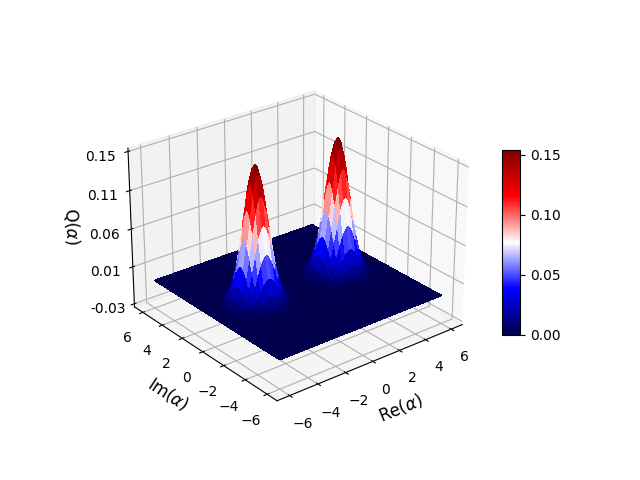
\includegraphics[scale=0.8]{542HW4/b1Q}
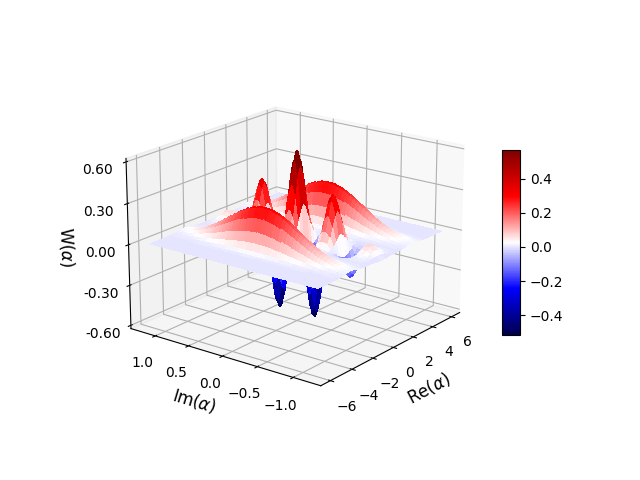
\includegraphics[scale=0.8]{542HW4/b1W}
\end{center}
\newpage

\textbf{(2) $\beta_2 = 3i$}. Note that the $\Re(\alpha)$-axis is re-scaled for the $W(\alpha)$ plot. 
\begin{center}
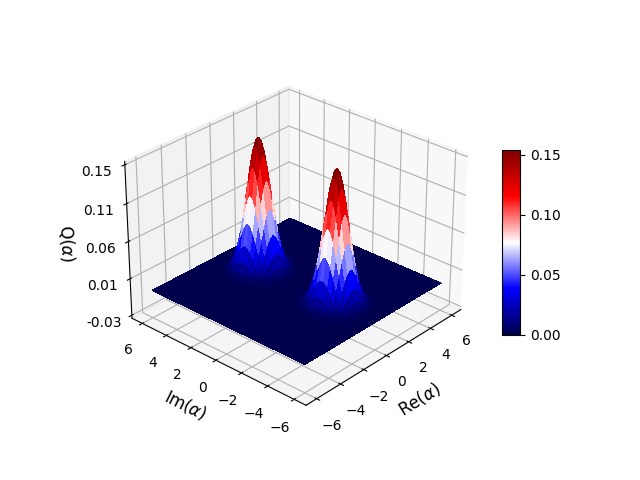
\includegraphics[scale=0.8]{542HW4/b2Q}
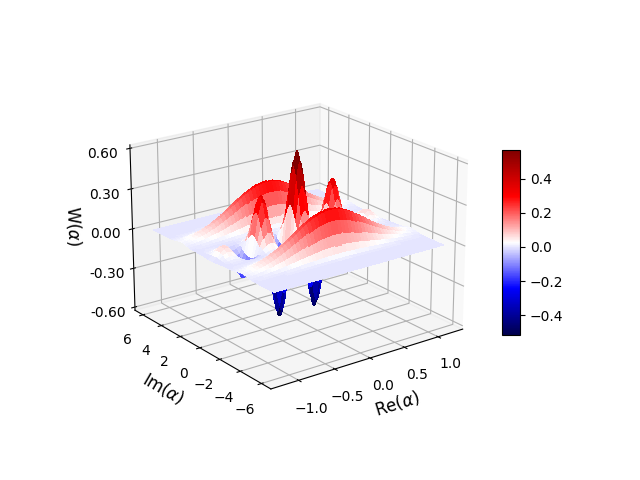
\includegraphics[scale=0.8]{542HW4/b2W}
\end{center}
\newpage

\textbf{(3) $\beta_3 = 3(1+i)/2$}. 
\begin{center}
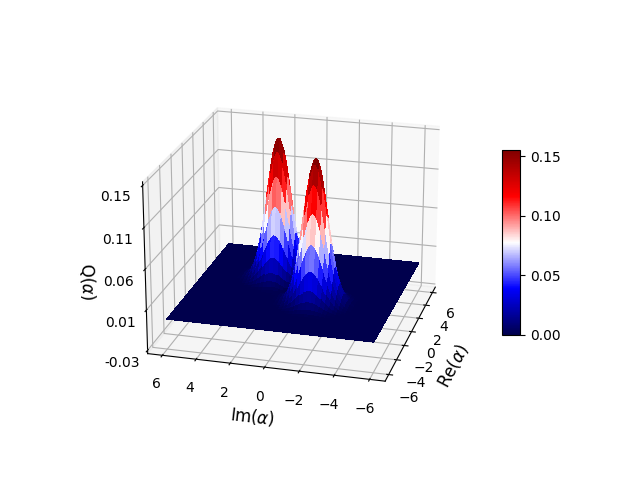
\includegraphics[scale=0.8]{542HW4/b3Q}
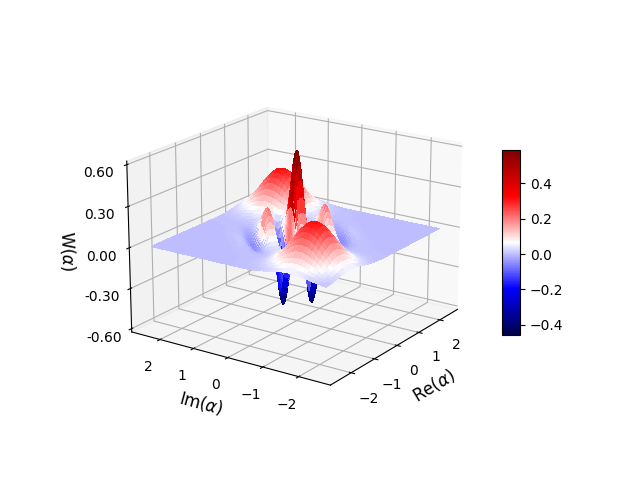
\includegraphics[scale=0.8]{542HW4/b3W}
\end{center}


\end{document}



